\documentclass[11pt,a4paper]{article}

\setlength{\textwidth}{17cm}
\setlength{\textheight}{24cm}
\setlength{\oddsidemargin}{-0.7cm}
\setlength{\evensidemargin}{-0.7cm}
\setlength{\topmargin}{0cm} 
\setlength{\headheight}{0cm}
\setlength{\headsep}{0cm}


\usepackage{color}
\usepackage[T1]{fontenc}
\usepackage[pdftex]{graphicx}
\usepackage{hyperref}
\usepackage{soul}
\usepackage{subfigure}

\newcommand\gerinput[1]{\textcolor{blue}{GA: #1}}
\newcommand\ncinput[1]{\textcolor{red}{NC: #1}}
\newcommand\pwtinput[1]{\textcolor{magenta}{PT: #1}}
\newcommand\projecttitle[0]{\textcolor{blue}{ROSIE}}

\newcommand\red[1]{\textcolor{red}{#1}}
\newcommand\magenta[1]{\textcolor{magenta}{#1}}

\usepackage{helvet}
\renewcommand{\familydefault}{\sfdefault}

\begin{document}

\title{Discussion}
\author{Isaac Jordon, Natalia Chechina, Gerardo Aragon Camarasa, and Phil Trinder}

\maketitle


%%---------------------------------------------------

\section{Experiment 1}
\label{sec:exp1}

\begin{figure*}%[!t]
     \begin{center}
        \subfigure[10,000Hz]{%
           \label{fig:exp1-msg-latency-10khz}
           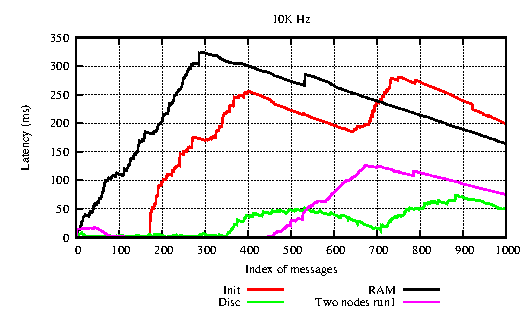
\includegraphics[width=0.49\textwidth]{gnuplot/exp1-msg-latency-10khz.pdf}
        }\hspace*{3mm}
        \subfigure[100,000Hz]{%
            \label{fig:exp1-msg-latency-100khz}
           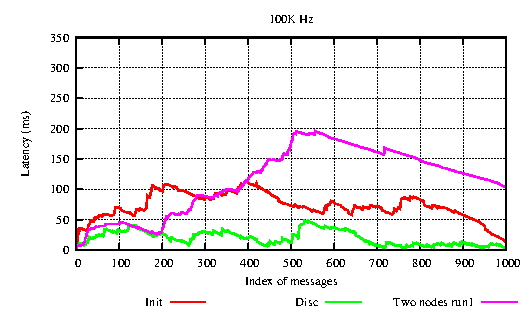
\includegraphics[width=0.49\textwidth]{gnuplot/exp1-msg-latency-100khz.pdf}
        }\\
        \subfigure[1000,000Hz]{%
            \label{fig:exp1-msg-latency-100khz}
           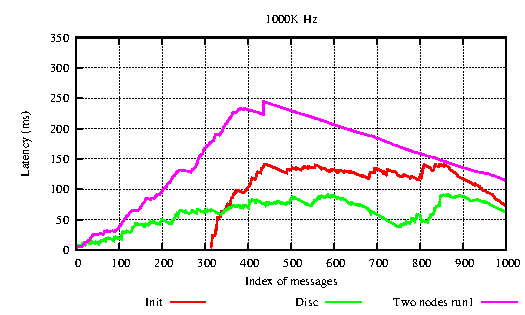
\includegraphics[width=0.49\textwidth]{gnuplot/exp1-msg-latency-1000khz.pdf}
        }
    \end{center}
    \caption{Message Latency}
   \label{fig:exp1-msg-latency}
\end{figure*}


\begin{figure*}%[!t]
     \begin{center}
        \subfigure[10,000Hz]{%
           \label{fig:exp1-msg-latency-10khz}
           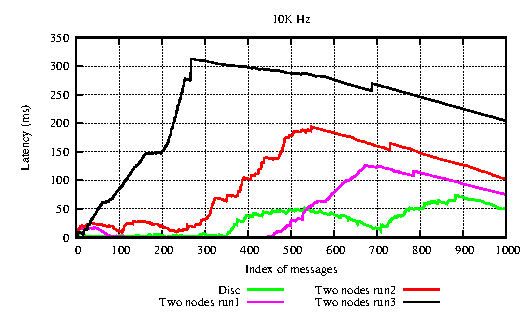
\includegraphics[width=0.49\textwidth]{gnuplot/exp1-msg-latency-two-10khz.pdf}
        }\hspace*{3mm}
        \subfigure[100,000Hz]{%
            \label{fig:exp1-msg-latency-100khz}
           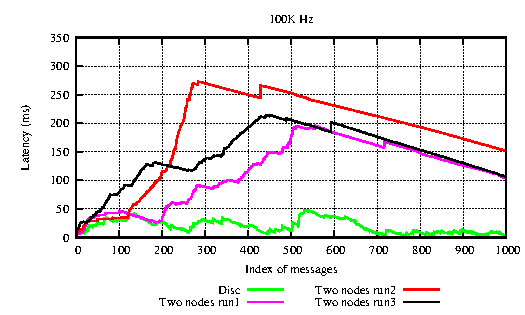
\includegraphics[width=0.49\textwidth]{gnuplot/exp1-msg-latency-two-100khz.pdf}
        }\\
        \subfigure[1000,000Hz]{%
            \label{fig:exp1-msg-latency-100khz}
           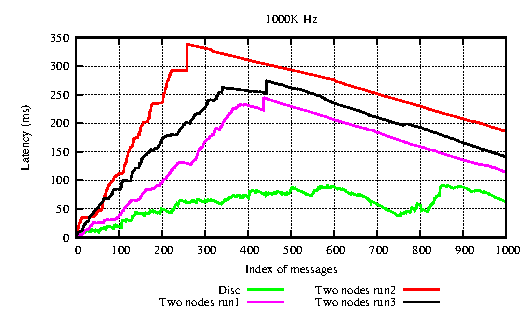
\includegraphics[width=0.49\textwidth]{gnuplot/exp1-msg-latency-two-1000khz.pdf}
        }
    \end{center}
    \caption{Message Latency (Two ROS nodes on Pi-1)}
   \label{fig:exp1-msg-latency-two}
\end{figure*}




%%~~~~~~~~~~~~~~~~~~~~~~~~~~~~~~~~~~~~~~~~~~
%\newpage
%\bibliographystyle{alpha}
%\bibliography{bibliography}

\end{document}








